\providecommand{\main}{../../..}
\documentclass[\main/main.tex]{subfiles}
\begin{document}

\subsection{Esercizio 1}
Si consideri il seguente problema con due indicatori che rappresentano costi:

\begin{align*}
  \min f_1(x) & =\frac{1}{4}\rnd{x_1-4}^2 + \frac{1}{4}x_2^2 \\
  \min f_2(x) & = 2 -x_2                                     \\
  2x_1 + x_2  & \leq 5                                       \\
  x_1, x_2    & \geq 0
\end{align*}

Si determini la soluzione che si avrebbe ipotizzando una funzione di utilit`a con
tasso marginale di sostituzione uniforme fra $f_1$ e $f_2$ e pesi $\w_1 = \frac{1}{3}$ e $\w_2 = \frac{2}{3}$.

\subsection{Soluzione esercizio 1}

\subsubsection*{Costruisco funzione obbiettivo composta}

\begin{align*}
  f^*(x) & =\frac{1}{3}\frac{1}{4}\rnd{\rnd{x_1-4}^2 + x_2^2} + \frac{2}{3}\rnd{2-x_2} \\
         & = \frac{1}{12}\rnd{\rnd{x_1-4}^2 + x_2^2} + \frac{2}{3}\rnd{2-x_2}          \\
         & = \frac{1}{12}\rnd{\rnd{x_1-4}^2 + x_2^2 + 8\rnd{2-x_2}}                    \\
         & = \frac{1}{12}\rnd{\rnd{x_1-4}^2 + x_2^2 + 16-8x_2}                         \\
         & = \frac{1}{12}\rnd{\rnd{x_1-4}^2 + \rnd{x_2-4}^2}                           \\
\end{align*}

\subsubsection*{Risolvo il problema}

Si tratta di una funzione distanza, con centro in $C = (4,4)$

\begin{align*}
  \min f^*(x) & = \frac{1}{12}\rnd{\rnd{x_1-4}^2 + \rnd{x_2-4}^2} \\
  2x_1 + x_2  & \leq 5                                            \\
  x_1, x_2    & \geq 0
\end{align*}

Il punto di ottimo è quello che giace sulla retta $2x_1+x_2=5$ più vicino al centro del cerchio $C = (4,4)$.

Ottengo la retta perpendicolare al vincolo passante per $C$:

\[
  g: x_2 = -2x_1 +5 \rightarrow m = -2, m' = \frac{1}{2} \Rightarrow  g': x_2 = \frac{1}{2}x_1 + q'
\]

Ottengo il termine costante della retta:

\[
  q' = 4 - \frac{1}{2}4 = 2
\]

La retta perpendicolare passante per $C$ risulta quindi:

\[
  -\frac{1}{2}x_1 + x_2 = 2
\]

Identifico quindi il punto più vicino a $C$ tramite l'intersezione delle due rette:

\[
  \begin{cases}
    -\frac{1}{2}x_1 + x_2 = 2 \\
    2x_1 + x_2  = 5
  \end{cases}
  \Rightarrow
  \begin{cases}
    x_2 = 2+\frac{3}{5} = \frac{13}{5} \\
    x_1 = \frac{6}{5}
  \end{cases}
\]

Il punto di ottimo risulta essere quindi $O = (\frac{6}{5}, \frac{13}{5})$

\subsubsection*{Verifico la soluzione}

\begin{figure}
  \begin{subfigure}{0.45\textwidth}
    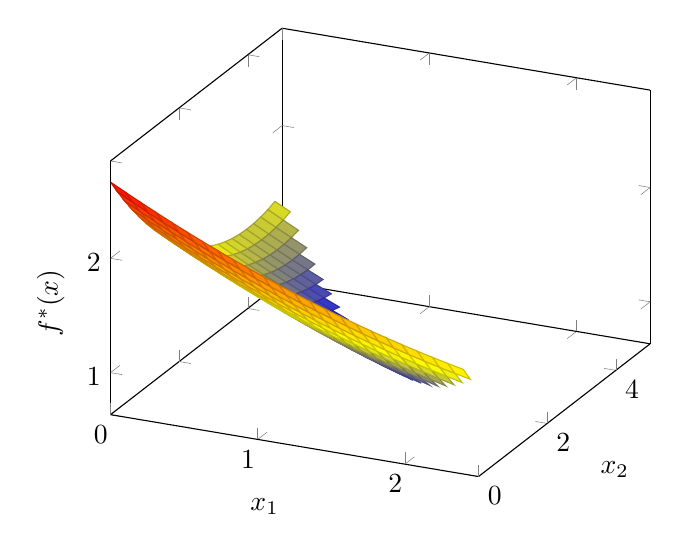
\begin{tikzpicture}
      \begin{axis}[
          xlabel=$x_1$,
          ylabel=$x_2$,
          zlabel=$f^*(x)$,
          domain=0:2.5,
          y domain=0:5
        ]
        \addplot3[surf, unbounded coords=jump]
        {2*x+y<=5 ? 1/12*((x-4)^2+(y-4)^2) : NaN};
      \end{axis}
    \end{tikzpicture}
    \caption{La funzione $f^*(x)$}
  \end{subfigure}
  ~
  \begin{subfigure}{0.45\textwidth}
    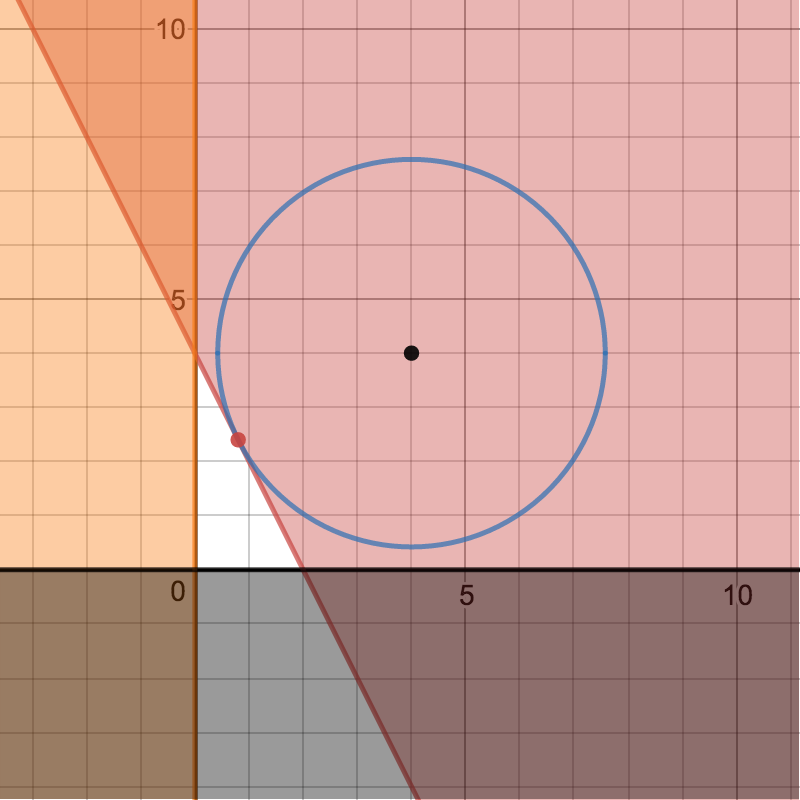
\includegraphics[width=0.8\textwidth]{es1-maut}
    \caption{Dominio della funzione $f^*(x)$}
  \end{subfigure}
\end{figure}

Il risultato ottenuto è valido.

\end{document}